\documentclass[12pt,a4paper]{article}
\usepackage[latin1]{inputenc}
\usepackage[spanish]{babel}
\usepackage{amsmath}
\usepackage{amsfonts}
\usepackage{amssymb}
\usepackage{pdfpages}
\usepackage{graphicx}
\usepackage[left=2cm,right=2cm,top=2cm,bottom=2cm]{geometry}
\begin{document}
\includepdf{CARATULA}
\title{\textbf{INFORME 2}}
\maketitle
El presente informe fue realizado con la finalidad de dar a conocer los cambios implementados en la aplicaci�n a ra�z de las correcciones realizadas por nuestro cliente (Docente) en el readme, a m�s de dar a conocer las nuevas implementaciones realizadas al recordatorio de voz con base en las planificaciones descritas en el backlog del producto.
\center{\large{\textbf{NUEVAS IMPLEMENTACIONES}}}

\begin{figure}[h!]
\begin{minipage}{0.5\textwidth}
\centering \includegraphics[width=0.75\textwidth]{1.png}    
\end{minipage}
\hfill\begin{minipage}{0.5\textwidth}
\textbf{Pantalla De Ver Recordatorio:  } Se agregaron las opciones de activar alarma y eliminar alarma, de las cuales activar alarma solo podr� ser utilizada si existe al menos un recordatorio grabado, y eliminar solo podr� ser utilizada en caso de que se haya definido una alarma. Ambas estar�n inactivas cuando no existan recordatorios.
\end{minipage}
\end{figure}

\begin{figure}[h!]
\begin{minipage}{0.5\textwidth}
\centering \includegraphics[width=0.75\textwidth]{2.png}     
\end{minipage}
\hfill\begin{minipage}{0.5\textwidth}
\textbf{Ventana de Activar Alarma: } Permite configurar la fecha y hora en que se desea recordar dicha informaci�n, adem�s del titulo que tendr� la alarma
\end{minipage}
\end{figure}

\begin{figure}[h!]
\begin{minipage}{0.5\textwidth}
\centering \includegraphics[width=0.75\textwidth]{3.png}      
\end{minipage}
\hfill\begin{minipage}{0.5\textwidth}
\textbf{Alarma activada: } Una vez que se haya guardado y activado la alarma, al momento que seleccionemos el recordatorio podr� ser visible los datos que se configuraron como: fecha, hora y titulo. 
\end{minipage}
\end{figure}

\pagebreak
Una vez que se ha mostrado espec�ficamente las modificaciones realizadas a las diferentes interfaces del reproductor Mp3, se procede a realizar el sprint de esta semana.

\newpage
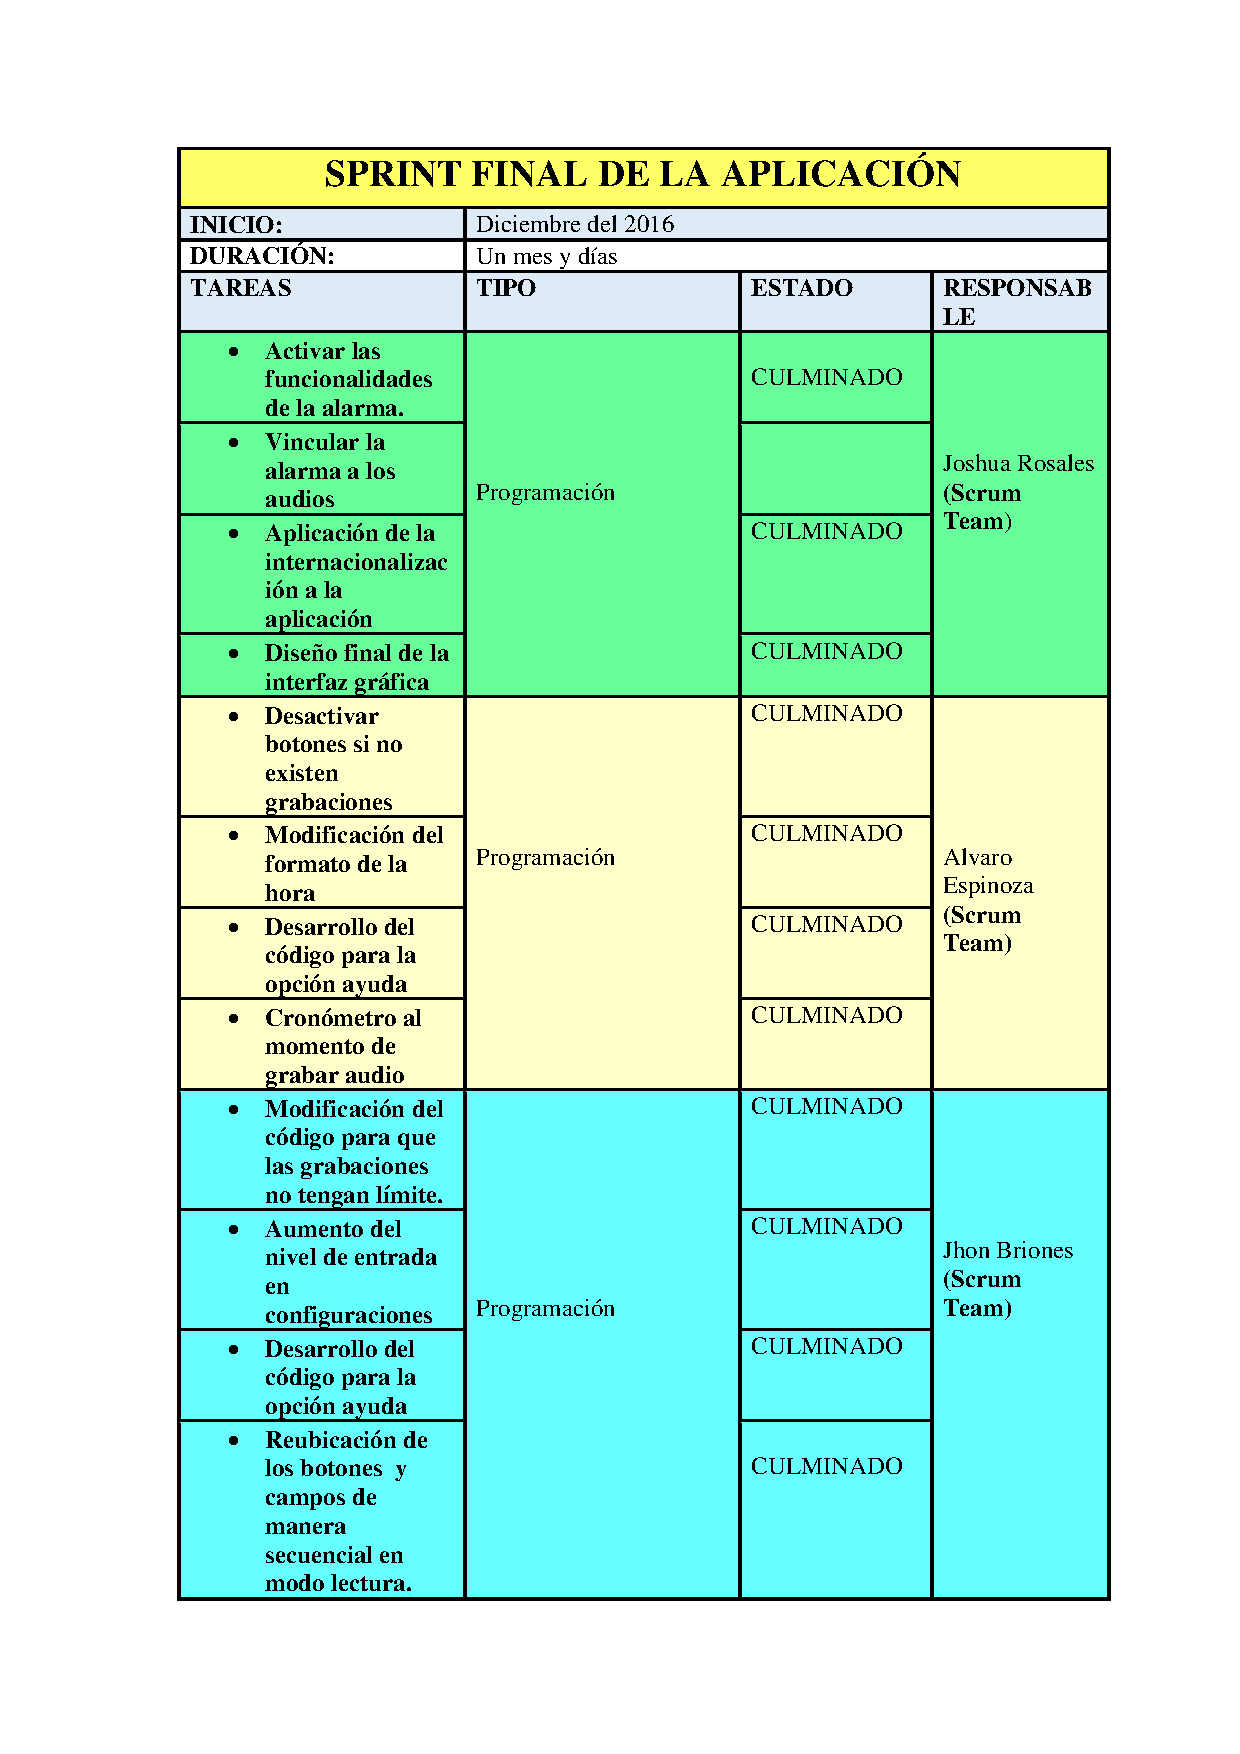
\includepdf{Sprint}
\end{document}